% fig11_tier_dist — integrated UFO verify-ledger tier distribution.
% Standalone pgfplots; compiled to figures/fig11_tier_dist.pdf.
% Comparison (tier distribution) => chart (user hard rule).
% Data: Appendix I, UFO/verify/V4_tier_ledger.md (companion/verify-ledger.json):
%   blue 8, green 11, yellow 8, orange 4, white 17, red 0.
\documentclass[border=4pt]{standalone}
\usepackage{tikz}
\usepackage{pgfplots}
\pgfplotsset{compat=1.18}
\begin{document}
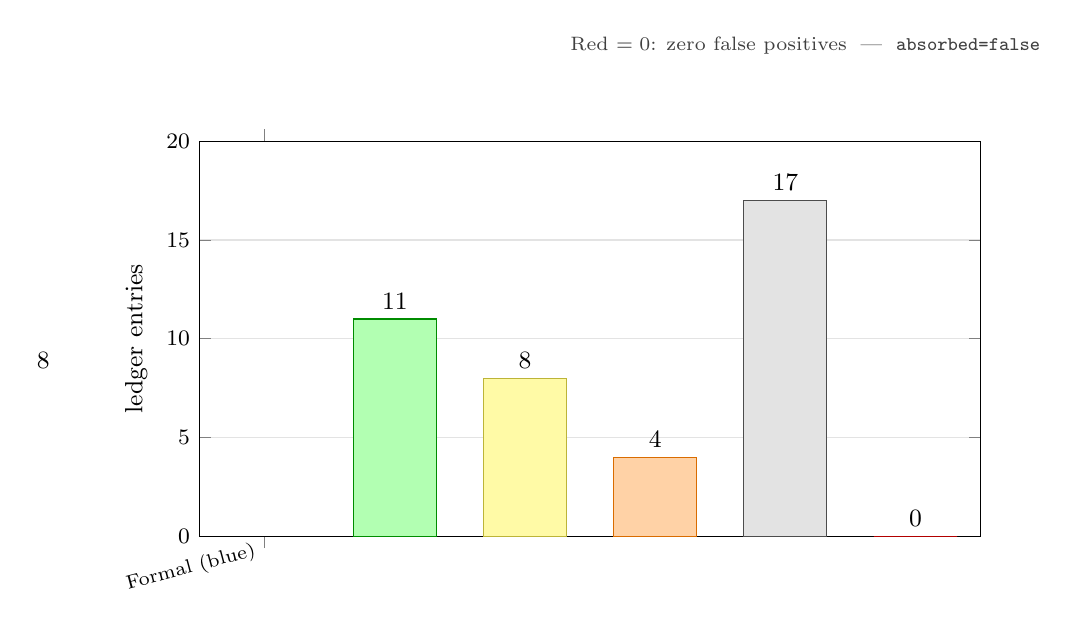
\begin{tikzpicture}
\begin{axis}[
  width=11.5cm, height=6.6cm,
  ybar,
  bar width=30pt,
  ymin=0, ymax=20,
  ylabel={ledger entries},
  symbolic x coords={Formal, Numerical, Cited, Deferred, Speculation, Falsified},
  xtick=data,
  xticklabels={Formal (blue), Numerical (green), Cited (yellow), Deferred (orange), Spec-Fenced (white), Falsified (red)},
  x tick label style={font=\scriptsize, rotate=15, anchor=east},
  tick label style={font=\footnotesize},
  label style={font=\small},
  nodes near coords,
  nodes near coords style={font=\small},
  ymajorgrids, grid style={gray!22},
  enlarge x limits=0.10,
]
\addplot[draw=blue!55!black,fill=blue!30] coordinates {(Formal,8)};
\addplot[draw=green!55!black,fill=green!30, bar shift=0pt] coordinates {(Numerical,11)};
\addplot[draw=yellow!70!black,fill=yellow!35, bar shift=0pt] coordinates {(Cited,8)};
\addplot[draw=orange!85!black,fill=orange!35, bar shift=0pt] coordinates {(Deferred,4)};
\addplot[draw=gray!60!black,fill=gray!22, bar shift=0pt] coordinates {(Speculation,17)};
\addplot[draw=red!70!black,fill=red!30, bar shift=0pt] coordinates {(Falsified,0)};
\end{axis}
\node[font=\scriptsize, gray!50!black, anchor=south east] at (10.8cm,6.0cm)
  {Red $=0$: zero false positives \;|\; \texttt{absorbed=false}};
\end{tikzpicture}
\end{document}
